\documentclass[journal]{IEEEtran}

\ifCLASSINFOpdf
  \usepackage[pdftex]{graphicx}
\else
  \usepackage[dvips]{graphicx}
\fi
\usepackage{mathtools, amssymb, amsfonts, mathrsfs, bm}
\usepackage{booktabs, multirow, makecell, adjustbox, colortbl, xcolor}
\usepackage{algorithm, algpseudocode}
\usepackage{url, float, pifont, soul, cancel}
\usepackage[caption=false]{subfig}
\usepackage[colorlinks=true,linkcolor=blue,
            citecolor=blue,urlcolor=blue,
            bookmarks=false]{hyperref}

\definecolor{bestgreen}{RGB}{144,238,144}
\definecolor{secondblue}{RGB}{173,216,230}
\newcommand{\best}[1]{\cellcolor{bestgreen}#1}
\newcommand{\second}[1]{\cellcolor{secondblue}#1}
\newcommand{\cmark}{\ding{51}}
\newcommand{\xmark}{\ding{55}}
\newtheorem{theorem}{Theorem}
\newtheorem{lemma}{Lemma}
\setlength{\fboxsep}{1pt}
\def\x{{\mathbf x}}
\def\L{{\cal L}}
\hyphenation{op-tical net-works semi-conduc-tor}

\begin{document}

\title{Camouflage Unlearning: Fast and Surgical Machine 
Unlearning for Biometric Systems}

%% ====================================================
%% PEER REVIEW VERSION — uncomment block below
%% Author names hidden for blind review — saves space!
%% ====================================================
% \author{Anonymous Authors}

%% ====================================================
%% FINAL / CAMERA-READY — uncomment block below
%% (comment out the block above first)
%% ====================================================
% \author{First~A.~Author,~\IEEEmembership{Member,~IEEE,}
%         Second~B.~Author,~\IEEEmembership{Member,~IEEE,}
%         and~Third~C.~Author~\IEEEmembership{Senior Member,~IEEE}%
% \thanks{This work was supported in part by [Funding Agency]
%         under Grant [Number].}
% \thanks{First A. Author is with [Department], [University],
%         [City, Country]. E-mail: first@university.edu}
% \thanks{Second B. Author is with [Department], [University],
%         [City, Country]. E-mail: second@university.edu}
% \thanks{Third C. Author is with [Department], [University],
%         [City, Country]. E-mail: third@university.edu}
% }

\markboth{IEEE Signal Processing Letters,~Vol.~XX, No.~XX, 2026}%
{Author \MakeLowercase{\textit{et al.}}: Camouflage Unlearning}

\maketitle

%% Abstract + Keywords
\begin{abstract}
Machine unlearning for privacy-critical biometric systems, fingerprint, iris, and face recognition, remains underexplored despite GDPR/CCPA mandates requiring erasure throughout deployment. Existing methods target classification and generative tasks, collapsing all forget classes to a single distant point, which inflates convergence time on resource-constrained edge devices facing frequent, minimal-replay removal requests; they are also benchmarked almost exclusively on ResNet/ViT for CIFAR/ImageNet, leaving biometric backbones untested. We propose Camouflage Unlearning (CU), which maps forget classes to nearby retain-class boundaries instead of a single point, reducing migration distance; this proximity target shapes only the training-time optimization objective, and we verify empirically that it does not induce elevated impostor matches against the assigned retain identity at verification time. CU achieves 3--4$\times$ faster convergence via retain-dominance constraints and localized regularization that surgically updates specific transformer blocks, while maintaining competitive retain accuracy. Across classification, iris, fingerprint, and face recognition, CU shows competitive performance and privacy behavior (MIA $\approx$ 0.5), supporting its effectiveness for regulatory-compliant, deep embedding-based biometric authentication.
\end{abstract}

\begin{IEEEkeywords}
Biometric recognition, data privacy, face recognition, GDPR, machine unlearning, vision transformers
\end{IEEEkeywords}

%% Keep for peer review, REMOVE for final version
\IEEEpeerreviewmaketitle

%% Main Sections
\section{Introduction}
\IEEEPARstart{M}{achine} unlearning (MU) has emerged as a critical research area~\cite{hou2025fixguard,ye2023stealthy}, addressing the imperative to prevent unauthorized data exploitation, eliminate harmful model behaviors, and safeguard user privacy~\cite{zhu2024privauditor}. The proliferation of AI misuse ranging from phishing generation and model inversion attacks to perpetuating misinformation has prompted regulatory frameworks~\cite{li2024model,prabhakar2025model,kahla2022label}. Frameworks like the General Data Protection Regulation (GDPR) and California Consumer Privacy Act (CCPA)~\cite{goldman2020introduction,data2018general} mandate that model service providers erase user data from learned representations upon request, establishing legal and ethical obligations for responsible AI deployment. Users possess the right to request data removal at any time, so per-request efficiency becomes a first-class concern.


Existing machine unlearning methods predominantly target image classification~\cite{wuerkaixi2025accurate} and generative tasks~\cite{wei2025emma}, with limited exploration of privacy-critical biometric systems. While face recognition~\cite{de2024unlearning,zakharov2026face,shivam2025cure} has received modest attention, fingerprint and iris recognition remains substantially less studied. This gap persists despite their sensitive nature and widespread deployment in authentication systems. Contemporary approaches rely primarily on KL divergence maximization~\cite{kurmanji2023towards} or gradient ascent~\cite{zhao2024continual}. These methods implement many-to-one mappings that force forgotten class embeddings toward a single distant point in feature space. Alternative strategies include saliency-based selection~\cite{fan2023salun}, geometric boundary manipulation~\cite{chen2023boundary}, perturbation-based forgetting~\cite{sun2024forget}, and meta-learning optimization~\cite{huang2024learning,shi2025mcu}. A key observation across all these methods is that every forget sample is driven toward a single collapse point in the decision space. Even when a sample already lies far from the retain manifold, it must still traverse the full distance to this distant target. This increases convergence time and GPU cost, as observed in Table~\ref{tab:all}. This many-to-one collapse behavior is visualized and ablated in detail in Section~\ref{sec:tsne}. Methods such as GS-LoRA~\cite{zhao2024continual}, SCRUB~\cite{kurmanji2023towards}, SalUn~\cite{fan2023salun}, Boundary Unlearning~\cite{chen2023boundary}, Forget Vectors~\cite{sun2024forget}, MCU~\cite{shi2025mcu}, LTU~\cite{huang2024learning}, DELETE~\cite{zhou2025decoupled}, LoTUS~\cite{spartalis2025lotus}, and MUNBa~\cite{wu2025munba} each trade off convergence speed, memory, or reversibility, and few explicitly target biometric edge deployment or sequential forget cycles.

Biometric recognition differs from general classification in ways that directly affect unlearning feasibility. Biometric systems deploy on resource-constrained edge devices. Removal requests arrive sequentially and frequently over the deployment lifecycle. This transforms unlearning into a recurring operational cost rather than a one-time procedure. Under this workload, existing many-to-one methods become prohibitive as per request compute scales poorly with request frequency. Compounding this, existing unlearning methods have been designed and benchmarked almost exclusively on ResNet~\cite{he2016deep} or ViT backbones~\cite{dosovitskiy2020image} for CIFAR~\cite{krizhevsky2009learning} and ImageNet~\cite{russakovsky2015imagenet}. Their transferability to biometric backbones remains untested, despite architectures such as Face Transformer~\cite{zhong2021face}, LAM~\cite{luo2025novel}, JIPNet~\cite{guan2024joint}, SSLDMNet-Iris~\cite{kadhim2025deep}, IrisFormer~\cite{sun2024irisformer}, PFSimNet~\cite{yu2024partial}, and MEM-FR~\cite{wu2025privacy} representing the state of the art among deep embedding-based biometric backbones. What biometric unlearning requires instead is a cycle-robust method validated directly on biometric backbones.

To address these challenges, we propose Camouflage Unlearning (CU), a novel framework that achieves 3--4$\times$ faster convergence while maintaining robust performance. Unlike existing many-to-one approaches, CU pushes forget-class embeddings toward the nearest retained class boundaries, effectively reducing migration distances. This proximity target governs only the training-time optimization objective, not final verification-level similarity. A naive reading might suggest CU induces impersonation of the nearest retain identity, but Section~\ref{sec:attack} empirically verifies that forget probes do not match their assigned retain centroid more often than chance, ruling out this concern. To perform surgical modifications and minimize collateral damage to retain classes, CU employs localized regularization concentrated in specific blocks of the neural network. Additional details are provided in Section~\ref{sec:4}.

Our main contributions are summarized as follows:
\begin{enumerate}
    \item Among the earliest studies of machine unlearning for privacy-critical deep embedding-based biometric systems, covering fingerprint, iris, and face recognition.
    \item Camouflage Unlearning, achieving $3$--$4\times$ faster convergence than SoTA methods with competitive retention accuracy and privacy guarantees.
    \item Empirical evaluation across biometric and classification domains showing CU concentrates updates in specific network blocks and remains effective under data-scarce replay.
\end{enumerate}

\begin{figure*}
    \centering
    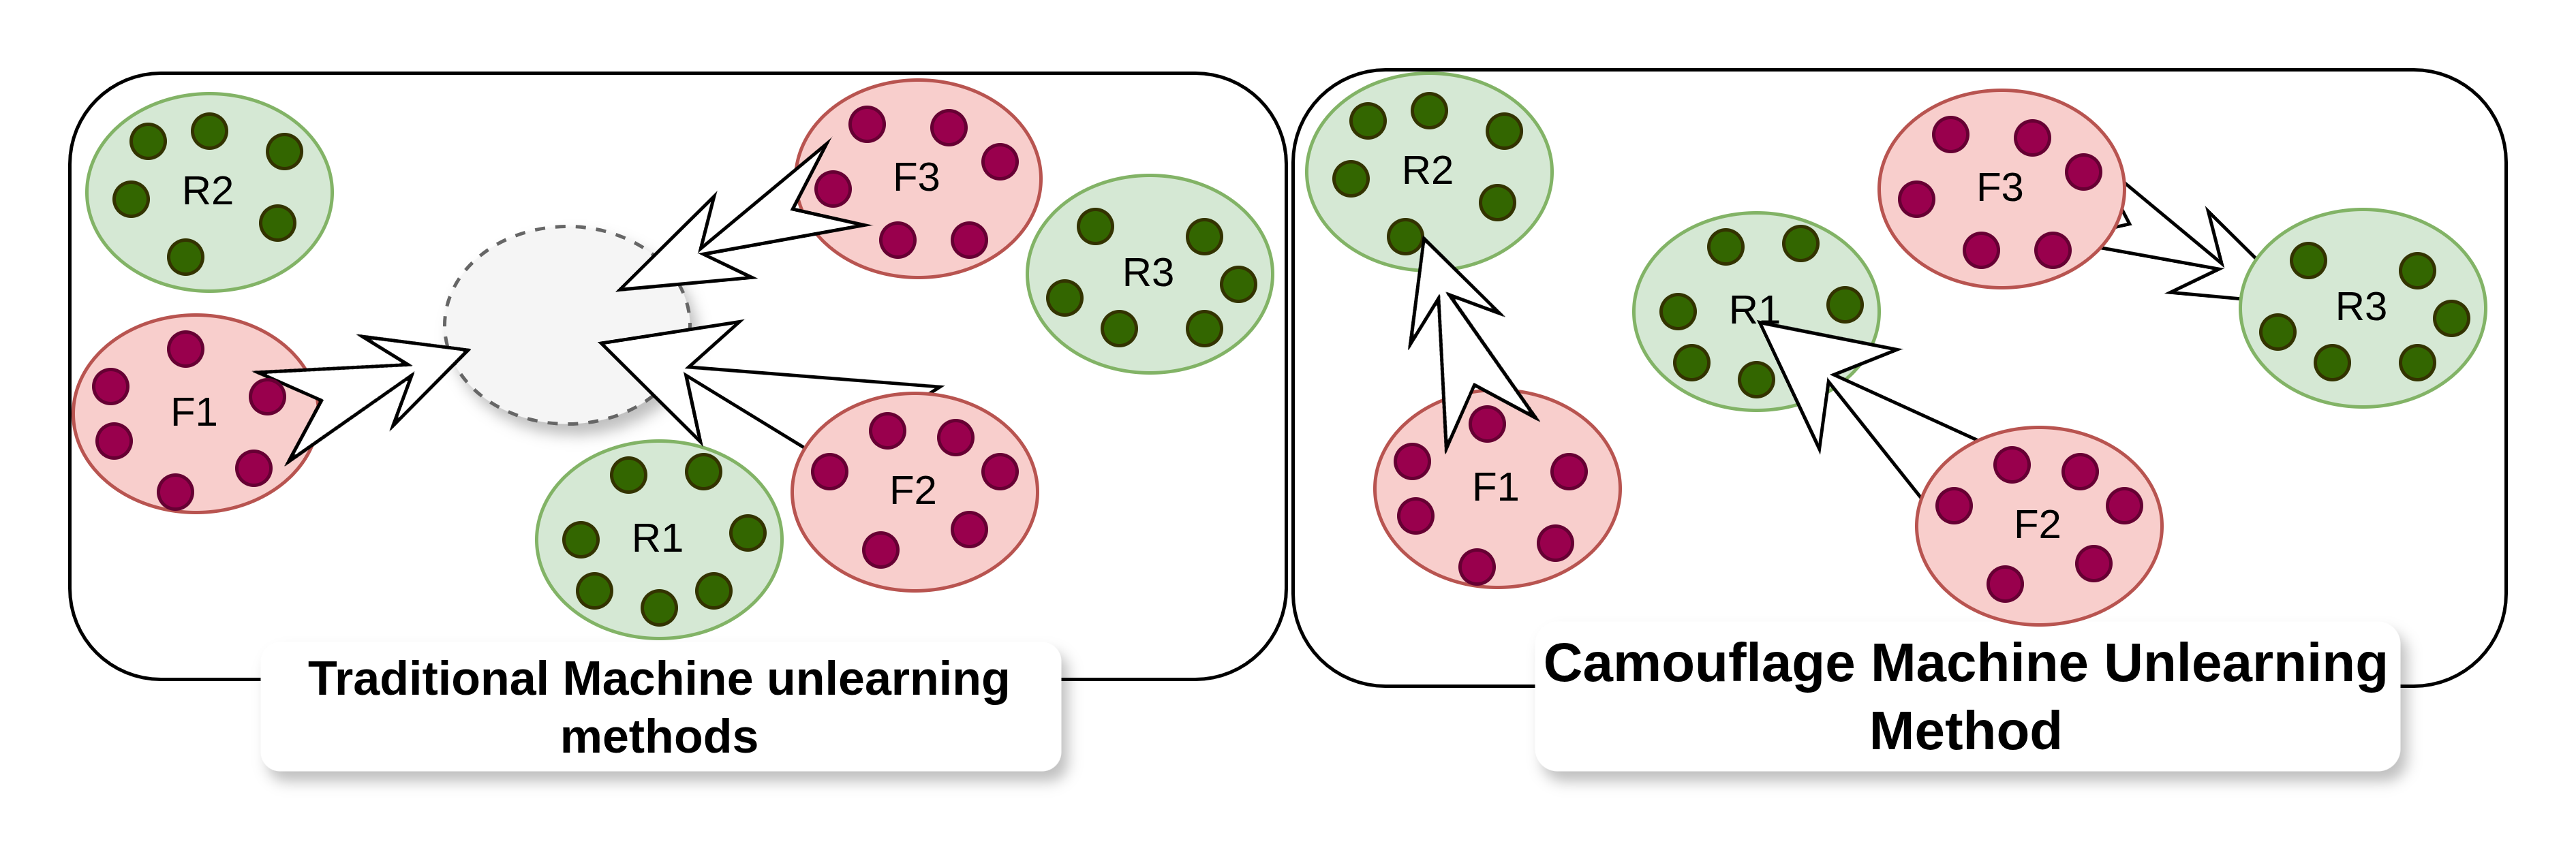
\includegraphics[width=1\textwidth]{images/Cam-Page-5.drawio.png}
    \caption{Overview of Camouflage Unlearning. Traditional methods collapse all forget classes to a single distant point, requiring long migration paths. CU instead hides each forget class within its nearest retain class boundary, reducing migration distance and accelerating convergence.}
    \label{fig:method}
\end{figure*}

\section{Problem Setting}
Let $\mathcal{M}$ be a model pre-trained on dataset $D$, representing a mapping $f_\mathcal{M} : \mathcal{X}_D \rightarrow \mathcal{Y}_D$ from input space $\mathcal{X}_D$ to output space $\mathcal{Y}_D$. Our objective is to selectively discard certain knowledge while preserving remaining knowledge. We partition the data as $D = D_\textit{r}^{\textit{full}} \cup D_\textit{f}$, where $D_\textit{f}$ denotes forget samples and $D_\textit{r}^{\textit{full}}$ denotes retain samples ($D_\textit{r}^{\textit{full}} \cap D_\textit{f} = \emptyset$).

In practice, storing the full retain set is prohibited under GDPR and CCPA regulations for privacy-sensitive data, while for non-private data, retraining remains computationally expensive due to large scale models and datasets. We therefore maintain a small replay buffer $D_\textit{r} \subset D_\textit{r}^{\textit{full}}$ such that $|D_\textit{r}| \ll |D_\textit{r}^{\textit{full}}|$, with $|D_\textit{r}|$ limited to at most 10\% of $|D_\textit{r}^{\textit{full}}|$\footnote{From this point, $D_\textit{r}$ denotes the replay buffer unless specified.}. Before unlearning, $\mathcal{M}$ performs well on $D_\textit{r}$ and $D_\textit{f}$, i.e.,
{\small
\begin{equation}
f_{\mathcal{M}} :
\mathcal{X}_{D_\textit{f}} \rightarrow \mathcal{Y}_{D_\textit{f}} \; ; \;
\mathcal{X}_{D_\textit{r}} \rightarrow \mathcal{Y}_{D_\textit{r}}
\label{eq:1}
\tag{1}
\end{equation}
}

Let the unlearning algorithm be $\mathcal{F}$ detailed in Section~\ref{sec:4}, which modifies model $\mathcal{M}$ to obtain $\mathcal{M}'$ via $\mathcal{M}' = \mathcal{F}(\mathcal{M}, D_\textit{f}, D_\textit{r})$. The unlearned model $\mathcal{M}'$ holds a new mapping $f_{\mathcal{M}'}$:
{\small
\begin{equation}
f_{\mathcal{M}'} :
\mathcal{X}_{D_\textit{f}} \cancel{\rightarrow} \mathcal{Y}_{D_\textit{f}} \; ; \;
\mathcal{X}_{D_\textit{r}} \rightarrow \mathcal{Y}_{D_\textit{r}}
\label{eq:2} \tag{2}
\end{equation}
}
Here, $\cancel{\rightarrow}$ denotes that the mapping no longer holds, i.e., the knowledge is forgotten, while $\rightarrow$ indicates the mapping persists. We define successful unlearning as 
\begin{itemize}
    \item Forgetting: $\textit{Acc}(\mathcal{M}', D_\textit{f}) \leq \frac{1}{C}, $
    \item Retention: $\textit{Acc}(\mathcal{M}', D_\textit{r}) \approx \textit{Acc}(\textit{Oracle}, D_\textit{r})$
\end{itemize}
where $C$ is the number of classes and Oracle denotes a model trained directly on target classes only.
\section{Performance Evaluation}
\subsection{Experimental Setup}

\noindent
\textbf{Datasets, Backbones, and Baselines:} We evaluate on CIFAR-100~\cite{krizhevsky2009learning} (DeiT-Tiny~\cite{touvron2021training}), CASIA-Iris~\cite{singh2017gender} (LAM~\cite{luo2025novel}), Sokoto Coventry fingerprints~\cite{shehu2018sokoto} (JIPNet~\cite{guan2024joint}), and CASIA-Face100~\cite{yi2014learning} (Face Transformer~\cite{zhong2021face}), comparing CU against SCRUB~\cite{kurmanji2023towards}, SalUn~\cite{fan2023salun}, GS-LoRA~\cite{zhao2024continual}, LTU~\cite{huang2024learning}, MCU~\cite{shi2025mcu}, and Forget Vectors~\cite{sun2024forget}, plus an Oracle trained only on $D_r^{\textbf{full}}$ as the upper bound.

\vspace{0.2cm}
\noindent
\textbf{Evaluation Metrics:} We report $Acc_f$, $Acc_r$, MIA (label-only attack~\cite{choquette2021label}, $\approx 0.5$ = safe), KL divergence to Oracle, RTE, and H-Mean~\cite{shibata2021learning}. Success requires $Acc_f \approx 0$, $Acc_r \approx$ Oracle, low KL/RTE. FAR@$\{0.3,0.4,0.5\}$/EER (cosine similarity, forget probes vs.\ retain gallery) further verify open-set identity confusion (Section~\ref{sec:attack}).

\subsection{Main Results}
\label{sec:main-results}
Table~\ref{tab:all} presents results across four tasks: classification, iris recognition, fingerprint recognition, and face recognition, where \colorbox{green!30}{green} highlights best performance and \colorbox{blue!30}{blue} indicates second-best.

\begin{table*}[!ht]
\centering
\small
\renewcommand{\arraystretch}{1.0}
\resizebox{\textwidth}{!}{%
\begin{tabular}{l|w{c}{1.1cm}w{c}{1.1cm}w{c}{1.1cm}w{c}{1.1cm}w{c}{1.1cm}w{c}{1.1cm}|w{c}{1.1cm}w{c}{1.1cm}w{c}{1.1cm}w{c}{1.1cm}w{c}{1.1cm}w{c}{1.1cm}}
\toprule
\multirow{2}{*}{\textbf{Method}}
& \multicolumn{6}{c|}{\textbf{Classification}} & \multicolumn{6}{c}{\textbf{Iris recognition}} \\
\cmidrule(lr){2-7} \cmidrule(lr){8-13}
& $Acc_f{\downarrow}$ & $Acc_r{\uparrow}$ & $H\text{-}Mean{\uparrow}$ & KL${\downarrow}$ & MIA$\downarrow$ & RTE${\downarrow}$
& $Acc_f{\downarrow}$ & $Acc_r{\uparrow}$ & $H\text{-}Mean{\uparrow}$ & KL${\downarrow}$ & MIA$\downarrow$ & RTE${\downarrow}$ \\
\midrule
Oracle        & --   & 77.36 & --    & --   & --   & --     & --   & 99.03 & --   & --   & --   & --    \\
\midrule
GS-LoRA~\cite{zhao2024continual}    & 0.11 & 71.32 & 74.18 & \colorbox{green!30}{0.73} & \colorbox{blue!30}{0.56} & \colorbox{blue!30}{153.2} & 0.00 & 93.42 & 96.18   & \colorbox{green!30}{0.75} & 0.69 & \colorbox{blue!30}{225.7} \\
SalUn~\cite{fan2023salun}           & 0.37 & 72.46 & 74.63 & 1.32 & 0.63 & 225.6 & 0.37 & 92.37 & 95.44 & \colorbox{blue!30}{0.79} & 0.59 & 427.2 \\
SCRUB~\cite{kurmanji2023towards}    & 0.58 & 73.11 & 74.90 & 1.89 & 0.64 & 219.3 & 0.43 & 95.58 & 97.07 & 0.83 & 0.63 & 501.8 \\
FV~\cite{sun2024forget}             & 0.00 & 74.43 & \colorbox{blue!30}{75.89} & 0.87 & \colorbox{green!30}{0.55} & 189.5 & 0.00 & 96.27 & 97.63   & 1.13 & 0.57 & 383.1 \\
MCU~\cite{shi2025mcu}               & 0.42 & 74.43 & 75.66 & 0.87 & 0.59 & {175.5} & 0.00 & \colorbox{green!30}{98.87} & \colorbox{green!30}{98.95}   & 0.99 & 0.63 & 437.2 \\
LTU~\cite{huang2024learning}        & 0.00 & \colorbox{green!30}{76.32} & \colorbox{green!30}{76.83} & \colorbox{green!30}{0.75} & 0.57 & 239.3 & 0.73 & 95.43 & 96.85 & 1.25 & \colorbox{blue!30}{0.55} & {329.4} \\
\midrule
\rowcolor{pink!15}
\textbf{CU}   & 0.47 & \colorbox{blue!30}{74.46} & 75.65 & {1.27} & \colorbox{blue!30}{0.56} & \colorbox{green!30}{55.5}  & 0.06 & \colorbox{blue!30}{97.89} & \colorbox{blue!30}{98.43} & 1.01 & \colorbox{green!30}{0.53} & \colorbox{green!30}{116.1} \\
\midrule
\addlinespace[0.15cm]
\midrule
\multirow{2}{*}{\textbf{Method}}
& \multicolumn{6}{c|}{\textbf{Fingerprint recognition}} & \multicolumn{6}{c}{\textbf{Face recognition}} \\
\cmidrule(lr){2-7} \cmidrule(lr){8-13}
& $Acc_f{\downarrow}$ & $Acc_r{\uparrow}$ & $H\text{-}Mean{\uparrow}$ & KL${\downarrow}$ & MIA$\downarrow$ & RTE${\downarrow}$
& $Acc_f{\downarrow}$ & $Acc_r{\uparrow}$ & $H\text{-}Mean{\uparrow}$ & KL${\downarrow}$ & MIA$\downarrow$ & RTE${\downarrow}$ \\
\midrule
Oracle        & --   & 90.82 & --    & -- & --   & --   & --   & 95.12   & --   & --   & --   & --   \\
\midrule
GS-LoRA~\cite{zhao2024continual}    & 0.00   & 83.42   & 86.98    & 1.13    & 0.65   & \colorbox{blue!30}{155.3}   & 0.57   & 93.25   & \colorbox{blue!30}{93.90}  & 1.13   & \colorbox{blue!30}{0.53}   & \colorbox{blue!30}{284.4}   \\
SalUn~\cite{fan2023salun}           & 0.10   & 82.32   & 86.24    & \colorbox{green!30}{0.75}    & 0.63   & 202.2   & 0.00   & 90.15   & 92.56  & 1.27   & 0.59   & 417.2   \\
SCRUB~\cite{kurmanji2023towards}    & 0.00   & 83.27   & 86.85    & 2.36    & 0.57   & 175.3   & 0.42   & \colorbox{blue!30}{93.27}   & 93.98  & 2.87   & 0.63   & 389.5   \\
FV~\cite{sun2024forget}             & 0.30   & 84.44   & 87.38    & 1.27    & \colorbox{green!30}{0.54}   & 160.7   & 0.20   & 92.27   & 93.58  & 1.20   & 0.60   & {380.3}   \\
MCU~\cite{shi2025mcu}               & 0.00   & 80.32   & 85.24    & \colorbox{blue!30}{0.99}    & 0.59   & 220.5   & 0.00   & 90.12   & 92.54  & \colorbox{green!30}{0.89}   & 0.57   & 403.8   \\
LTU~\cite{huang2024learning}        & 0.00   & \colorbox{green!30}{ 87.72}   & \colorbox{green!30}{89.24}    & 1.13    & \colorbox{green!30}{0.54}   & 237.4   & 0.00   & 92.58   & 93.84  & \colorbox{blue!30}{0.93}   & 0.55   & 430.2   \\
\midrule
\rowcolor{pink!15}
\textbf{CU}   & 0.00   & \colorbox{blue!30}{87.23}   & \colorbox{blue!30}{88.98}    & {1.05}    & \colorbox{blue!30}{0.55}   & \colorbox{green!30}{55.32}   & 0.00   & \colorbox{green!30}{93.98}   & \colorbox{green!30}{94.55}   & {1.67}   & \colorbox{green!30}{0.51}   & \colorbox{green!30}{175.3}   \\
\bottomrule
\end{tabular}%
}
\caption{Comprehensive performance evaluation across four recognition domains. Proposed CU achieves 3--4$\times$ speedup in runtime efficiency (RTE) while maintaining competitive forgetting, retention, and privacy metrics
.}
\label{tab:all}
\end{table*}

\vspace{0.2cm}
\noindent
\textbf{Unlearning and Retention:} All methods achieve near perfect forgetting $Acc_f < 1\%$, approaching random assignment. Proposed CU consistently ranks first or second in $Acc_r$ across all tasks, with LTU as the strongest competitor on classification, iris, and fingerprint tasks, while MCU excels on iris recognition. For \textit{H-Mean}, proposed CU alternates between first and second positions alongside competitive showings from LTU, FV, MCU, and GS-LoRA.

\vspace{0.2cm}
\noindent
\textbf{Privacy and Efficiency:} GS-LoRA achieves lower KL divergence than CU, which is expected since CU deliberately modifies logit distributions to suppress forget classes and is therefore less competitive on this metric. However, MIA scores near 0.5 confirm CU provides comparable privacy protection. Most critically, proposed CU achieves 3 to 4$\bm{\times}$ speedup versus all baselines, validating our design objective: fast, privacy-preserving unlearning without catastrophic forgetting.

\vspace{0.2cm}
\noindent
\textbf{Geometric Analysis of Unlearning Behavior:}
\label{sec:tsne}
To understand geometric behavior across unlearning methods, we visualize embedding space transformations using t-SNE. Figure~\ref{fig:tsne_comparison} compares baseline methods against proposed CU. Existing approaches GS-LoRA~\cite{zhao2024continual}, SCRUB~\cite{kurmanji2023towards}, and Boundary Unlearning~\cite{chen2023boundary} collapse forget classes into a single distant point, requiring long distance traversal in feature space. CU distributes forget samples across nearest retain class boundaries, achieving faster convergence through shorter migration paths, explaining the RTE gains in Table~\ref{tab:all}.

\begin{figure}[!ht]
    \centering
    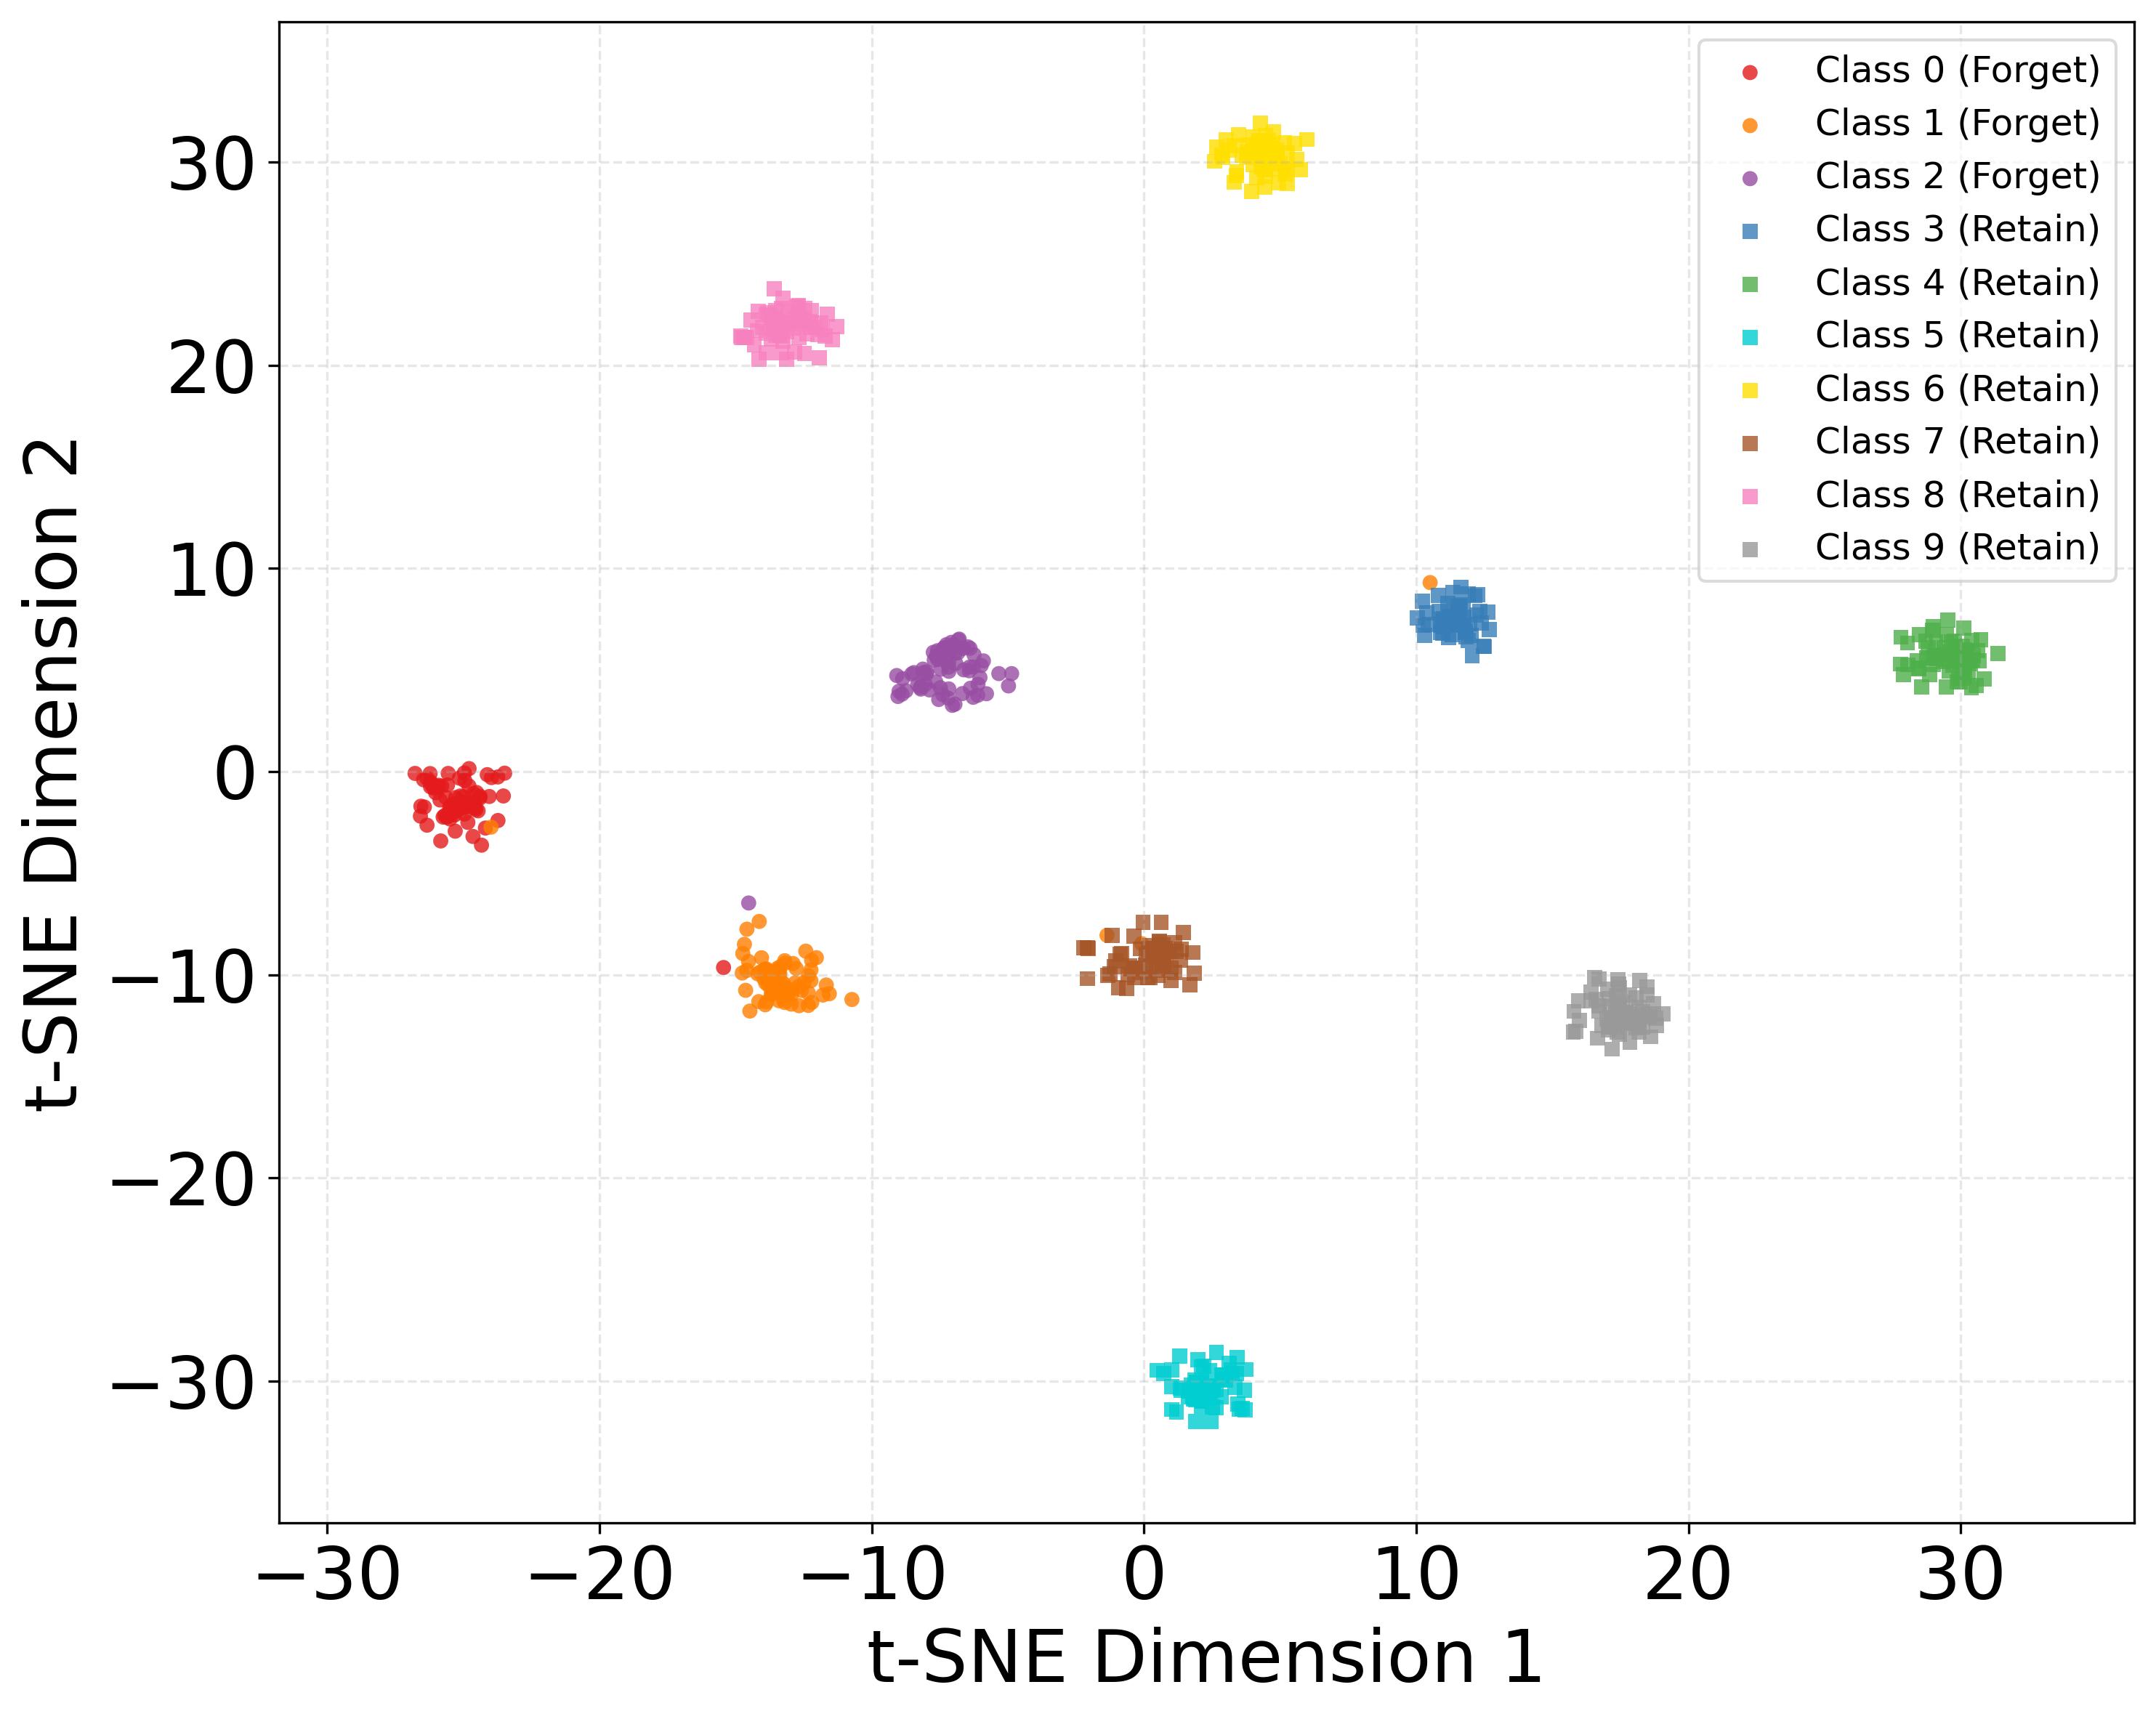
\includegraphics[width=0.45\linewidth]{tsne/base.png}
    \hfill
    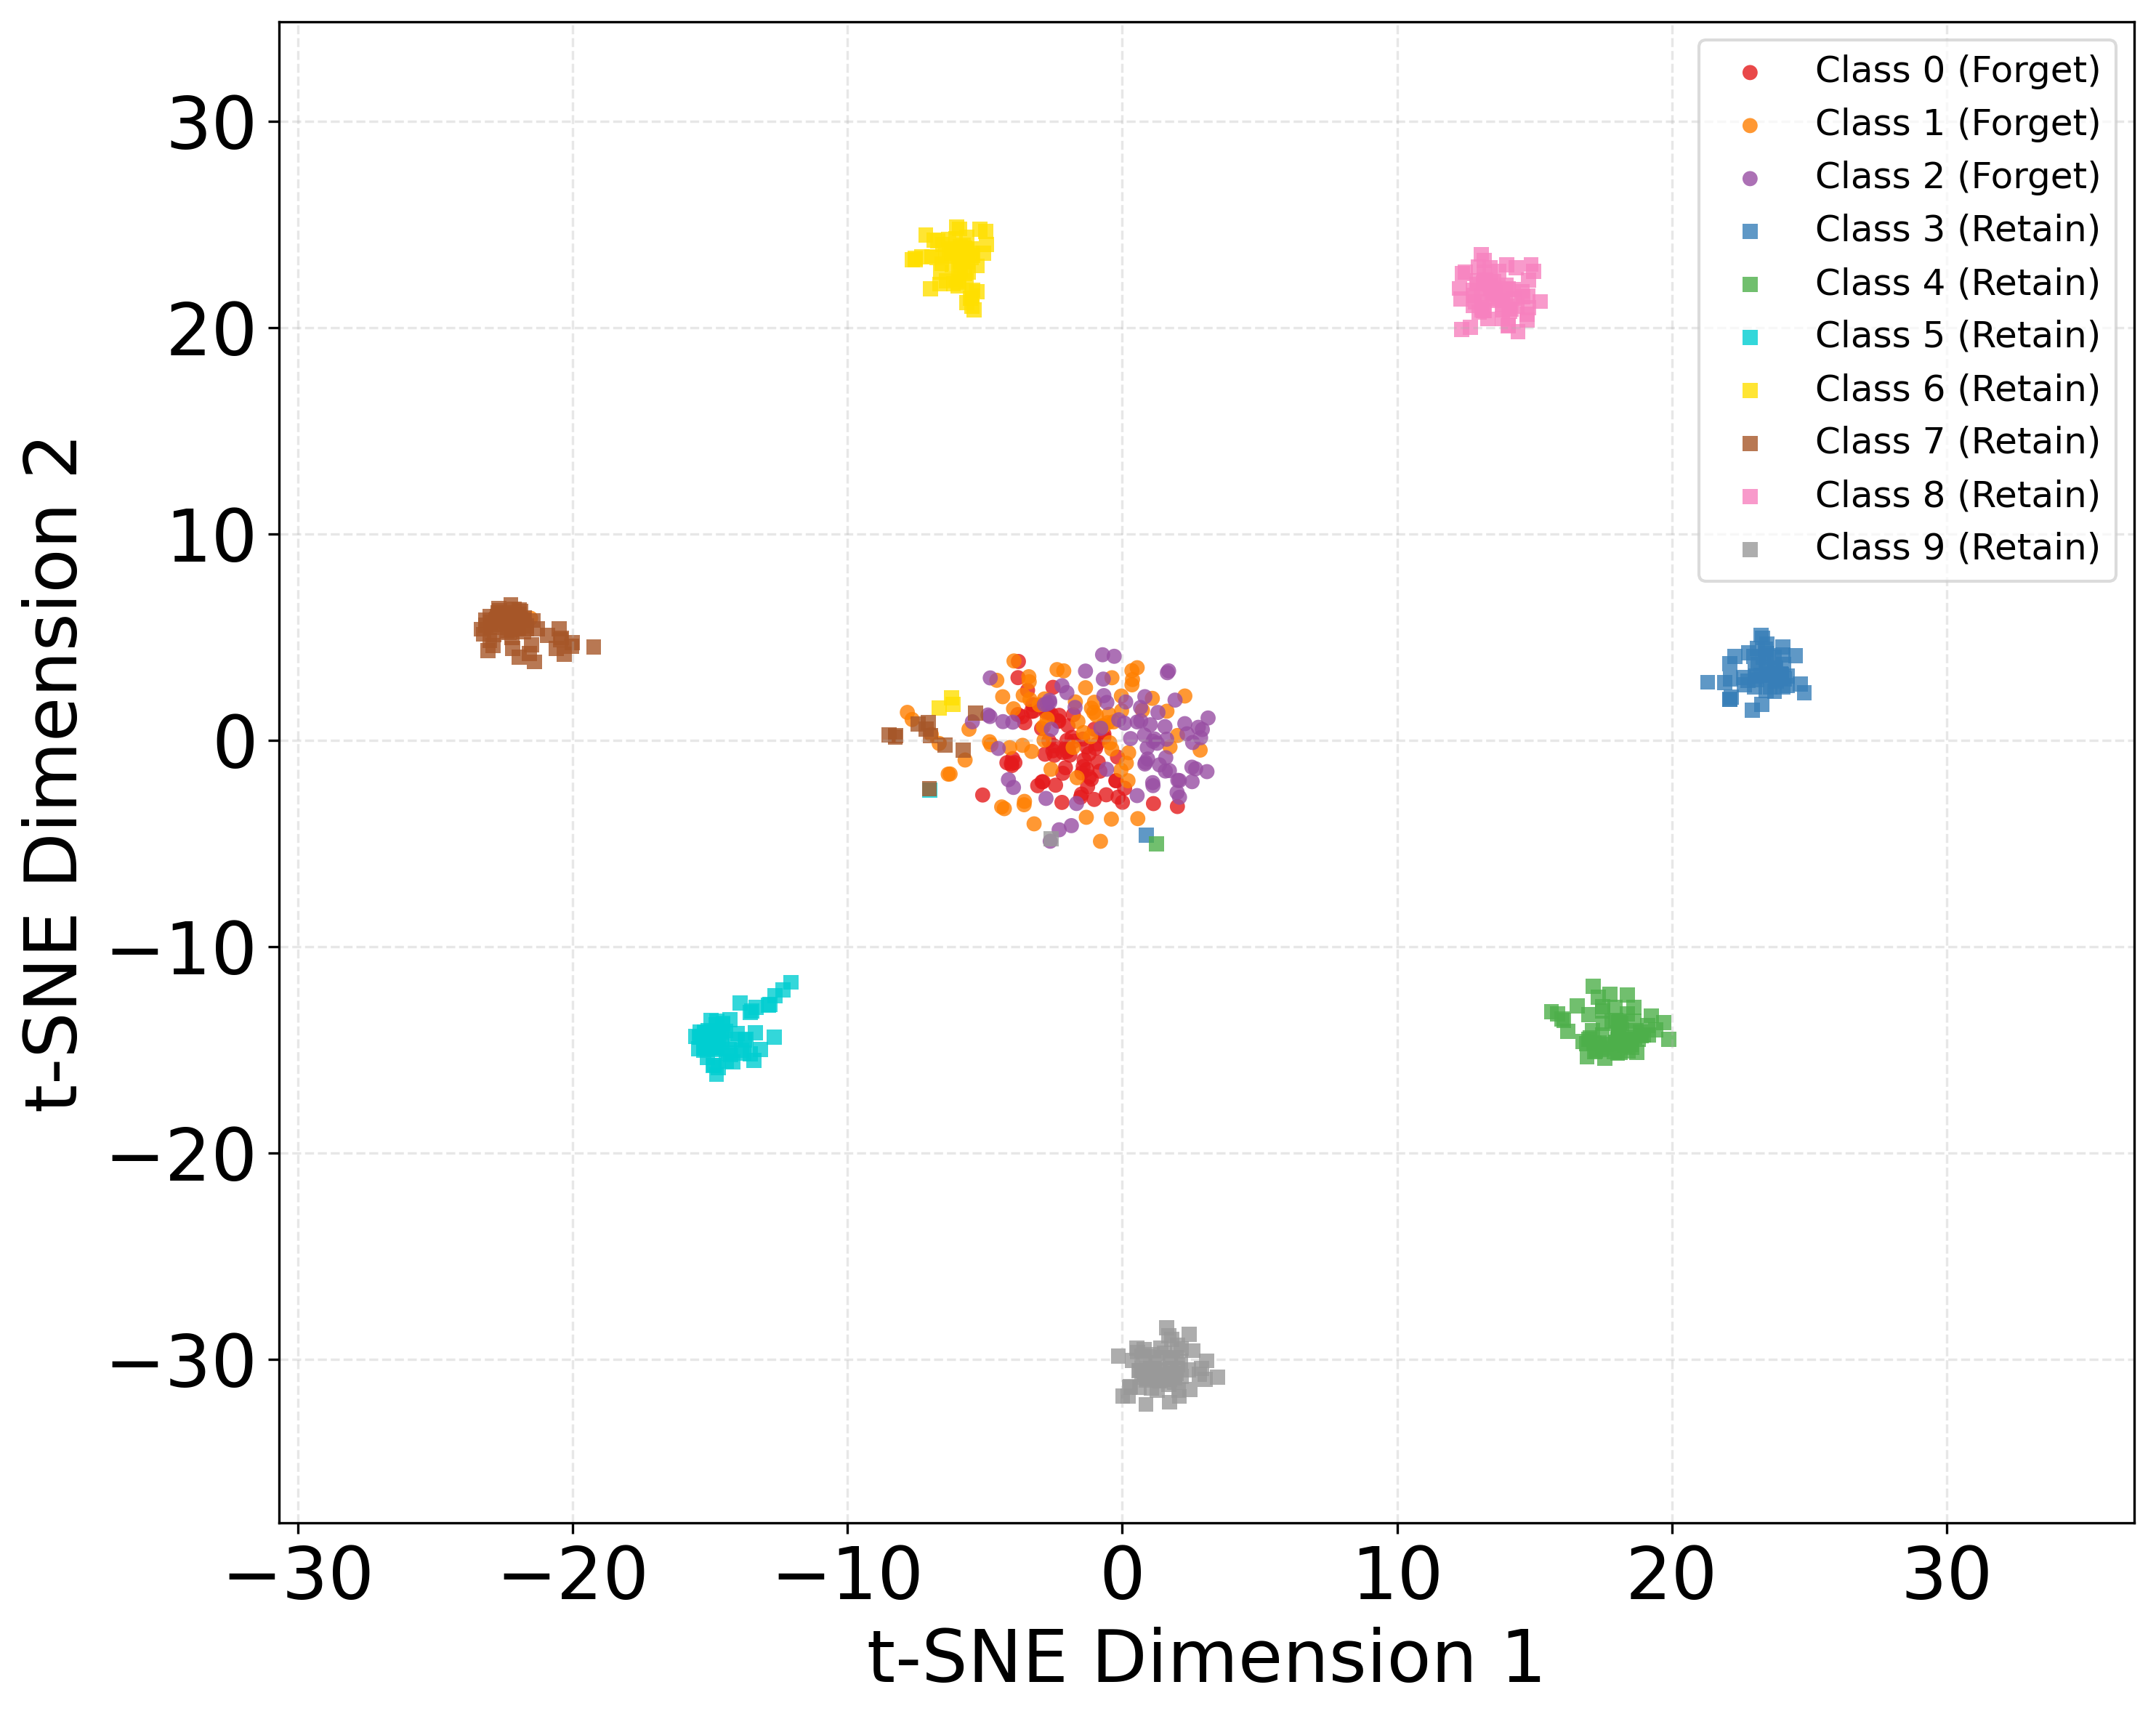
\includegraphics[width=0.45\linewidth]{tsne/GA.png}

    \vspace{0.3em}
    \makebox[0.45\linewidth]{\small (a) Initial}
    \hfill
    \makebox[0.45\linewidth]{\small (b) GS-LoRA}
    \vspace{1em}

    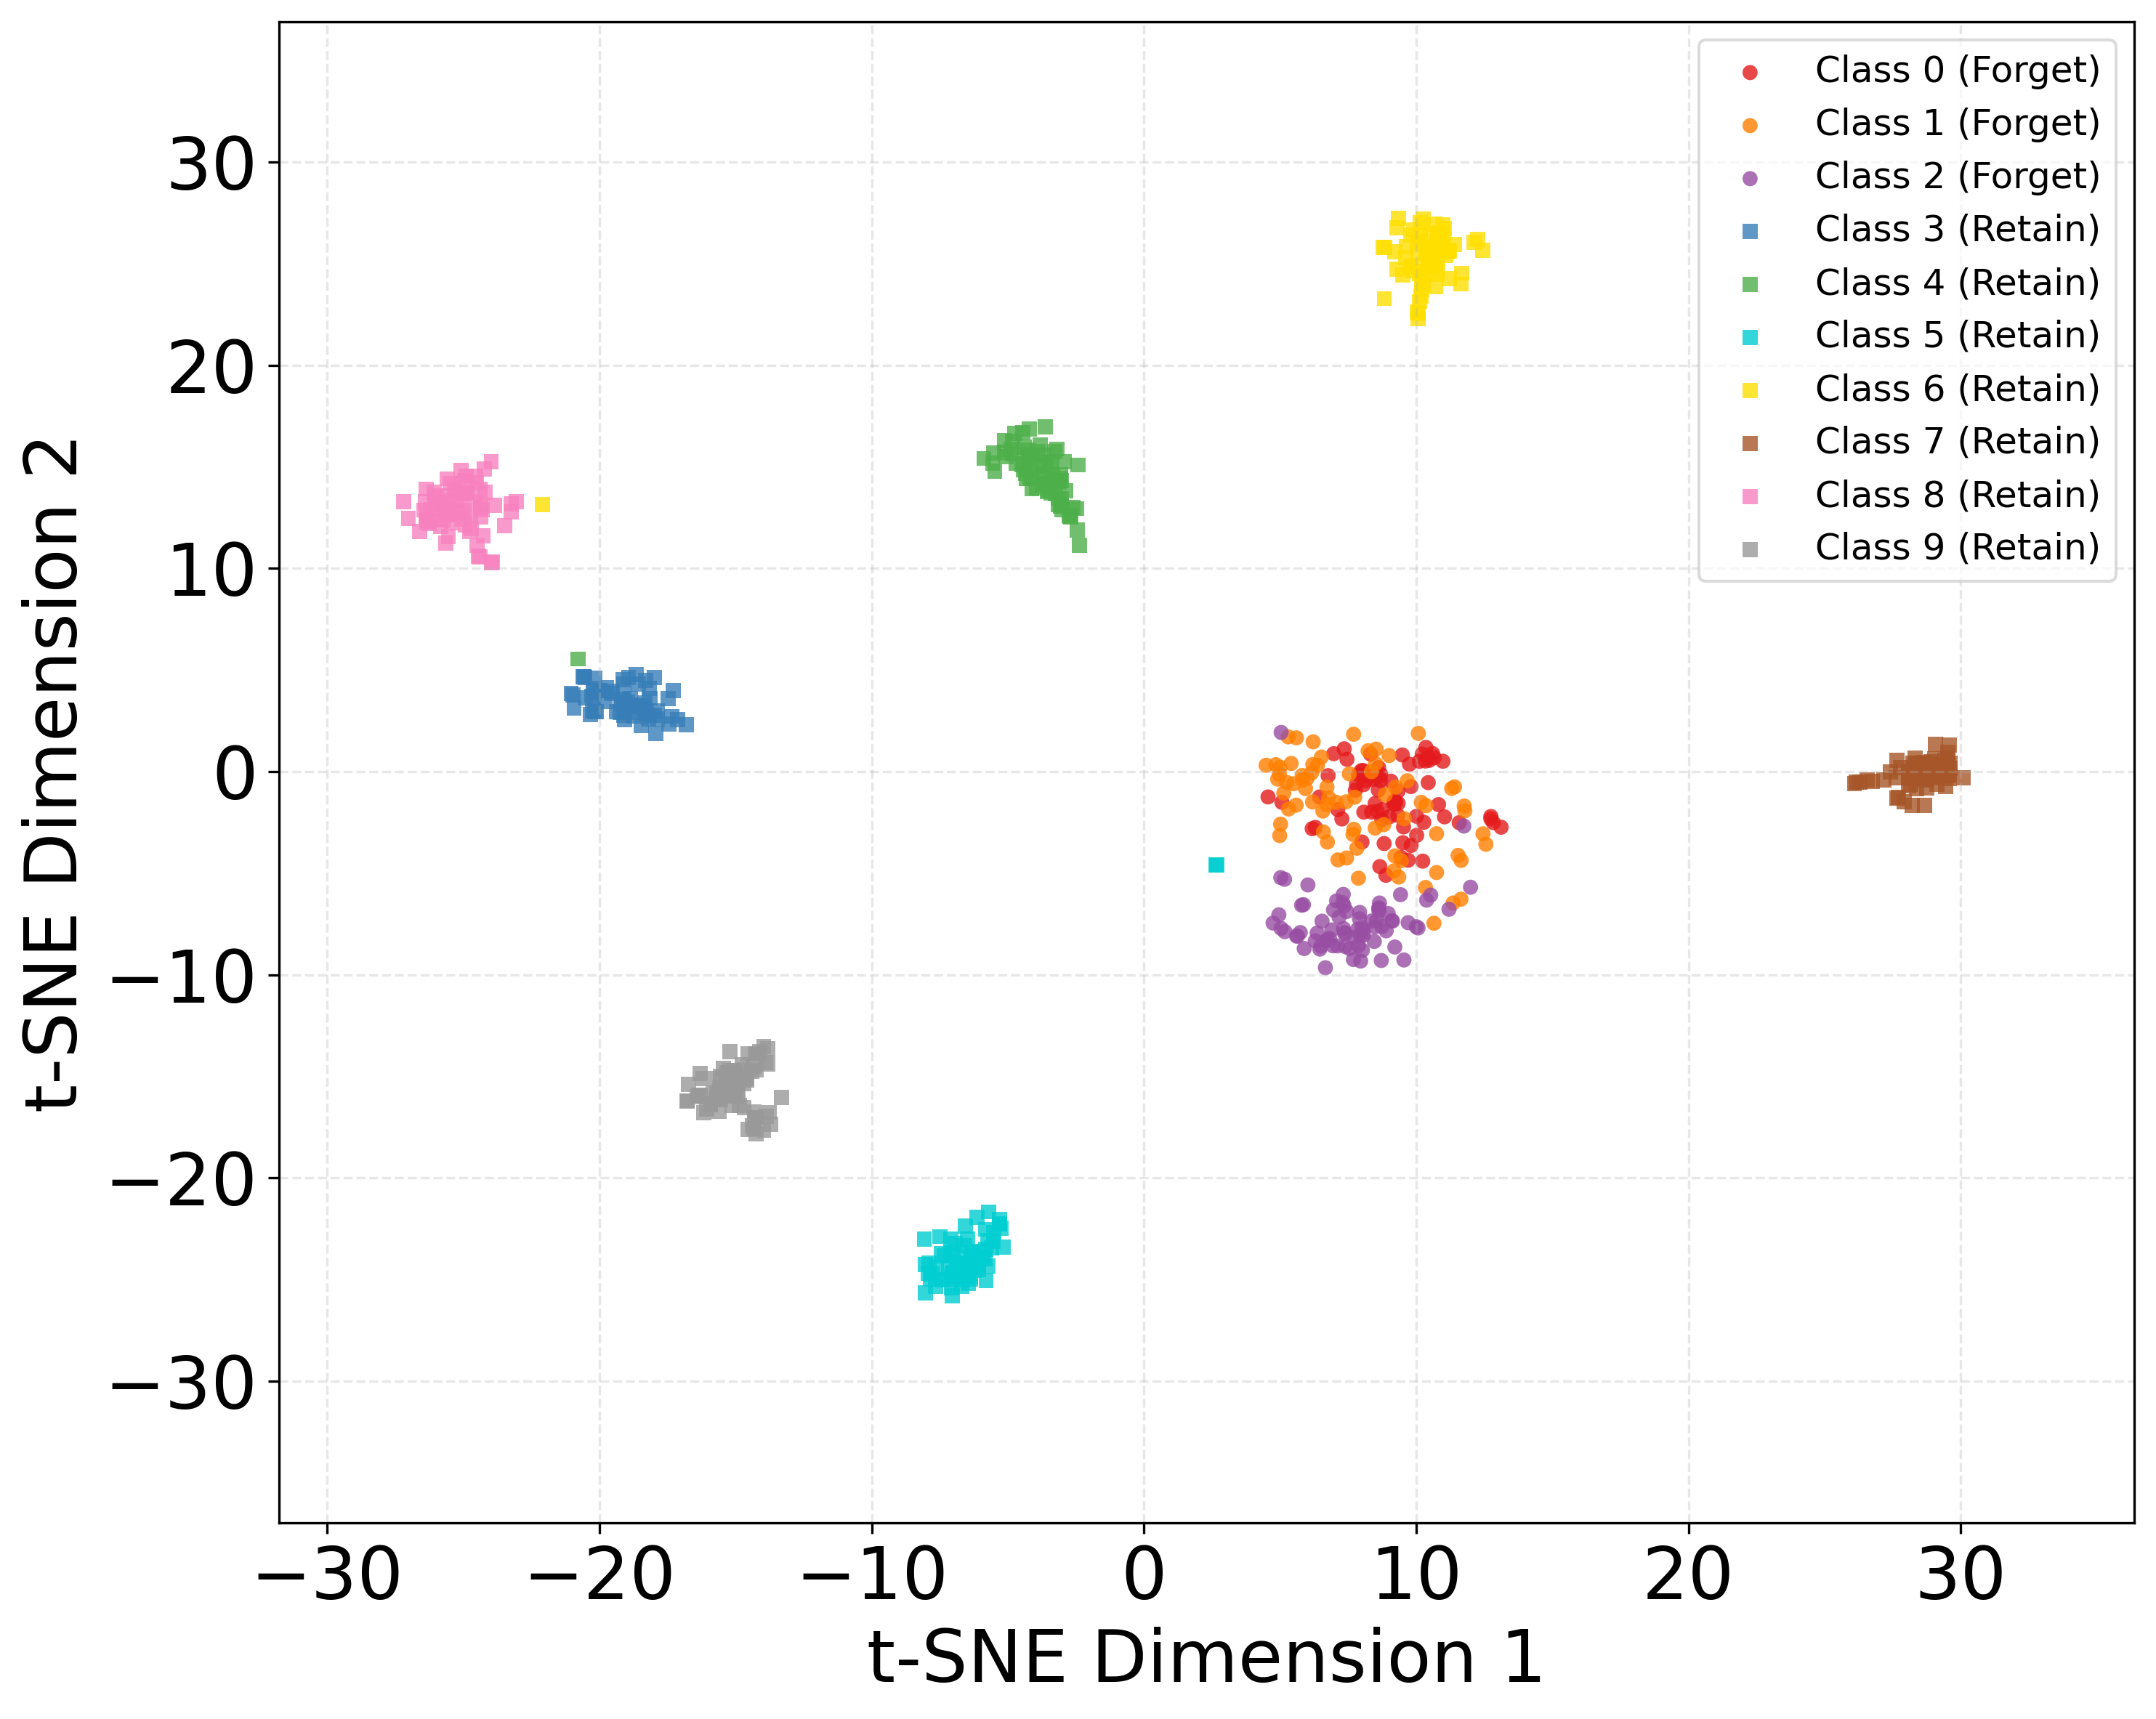
\includegraphics[width=0.45\linewidth]{tsne/shadow.png}
    \hfill
    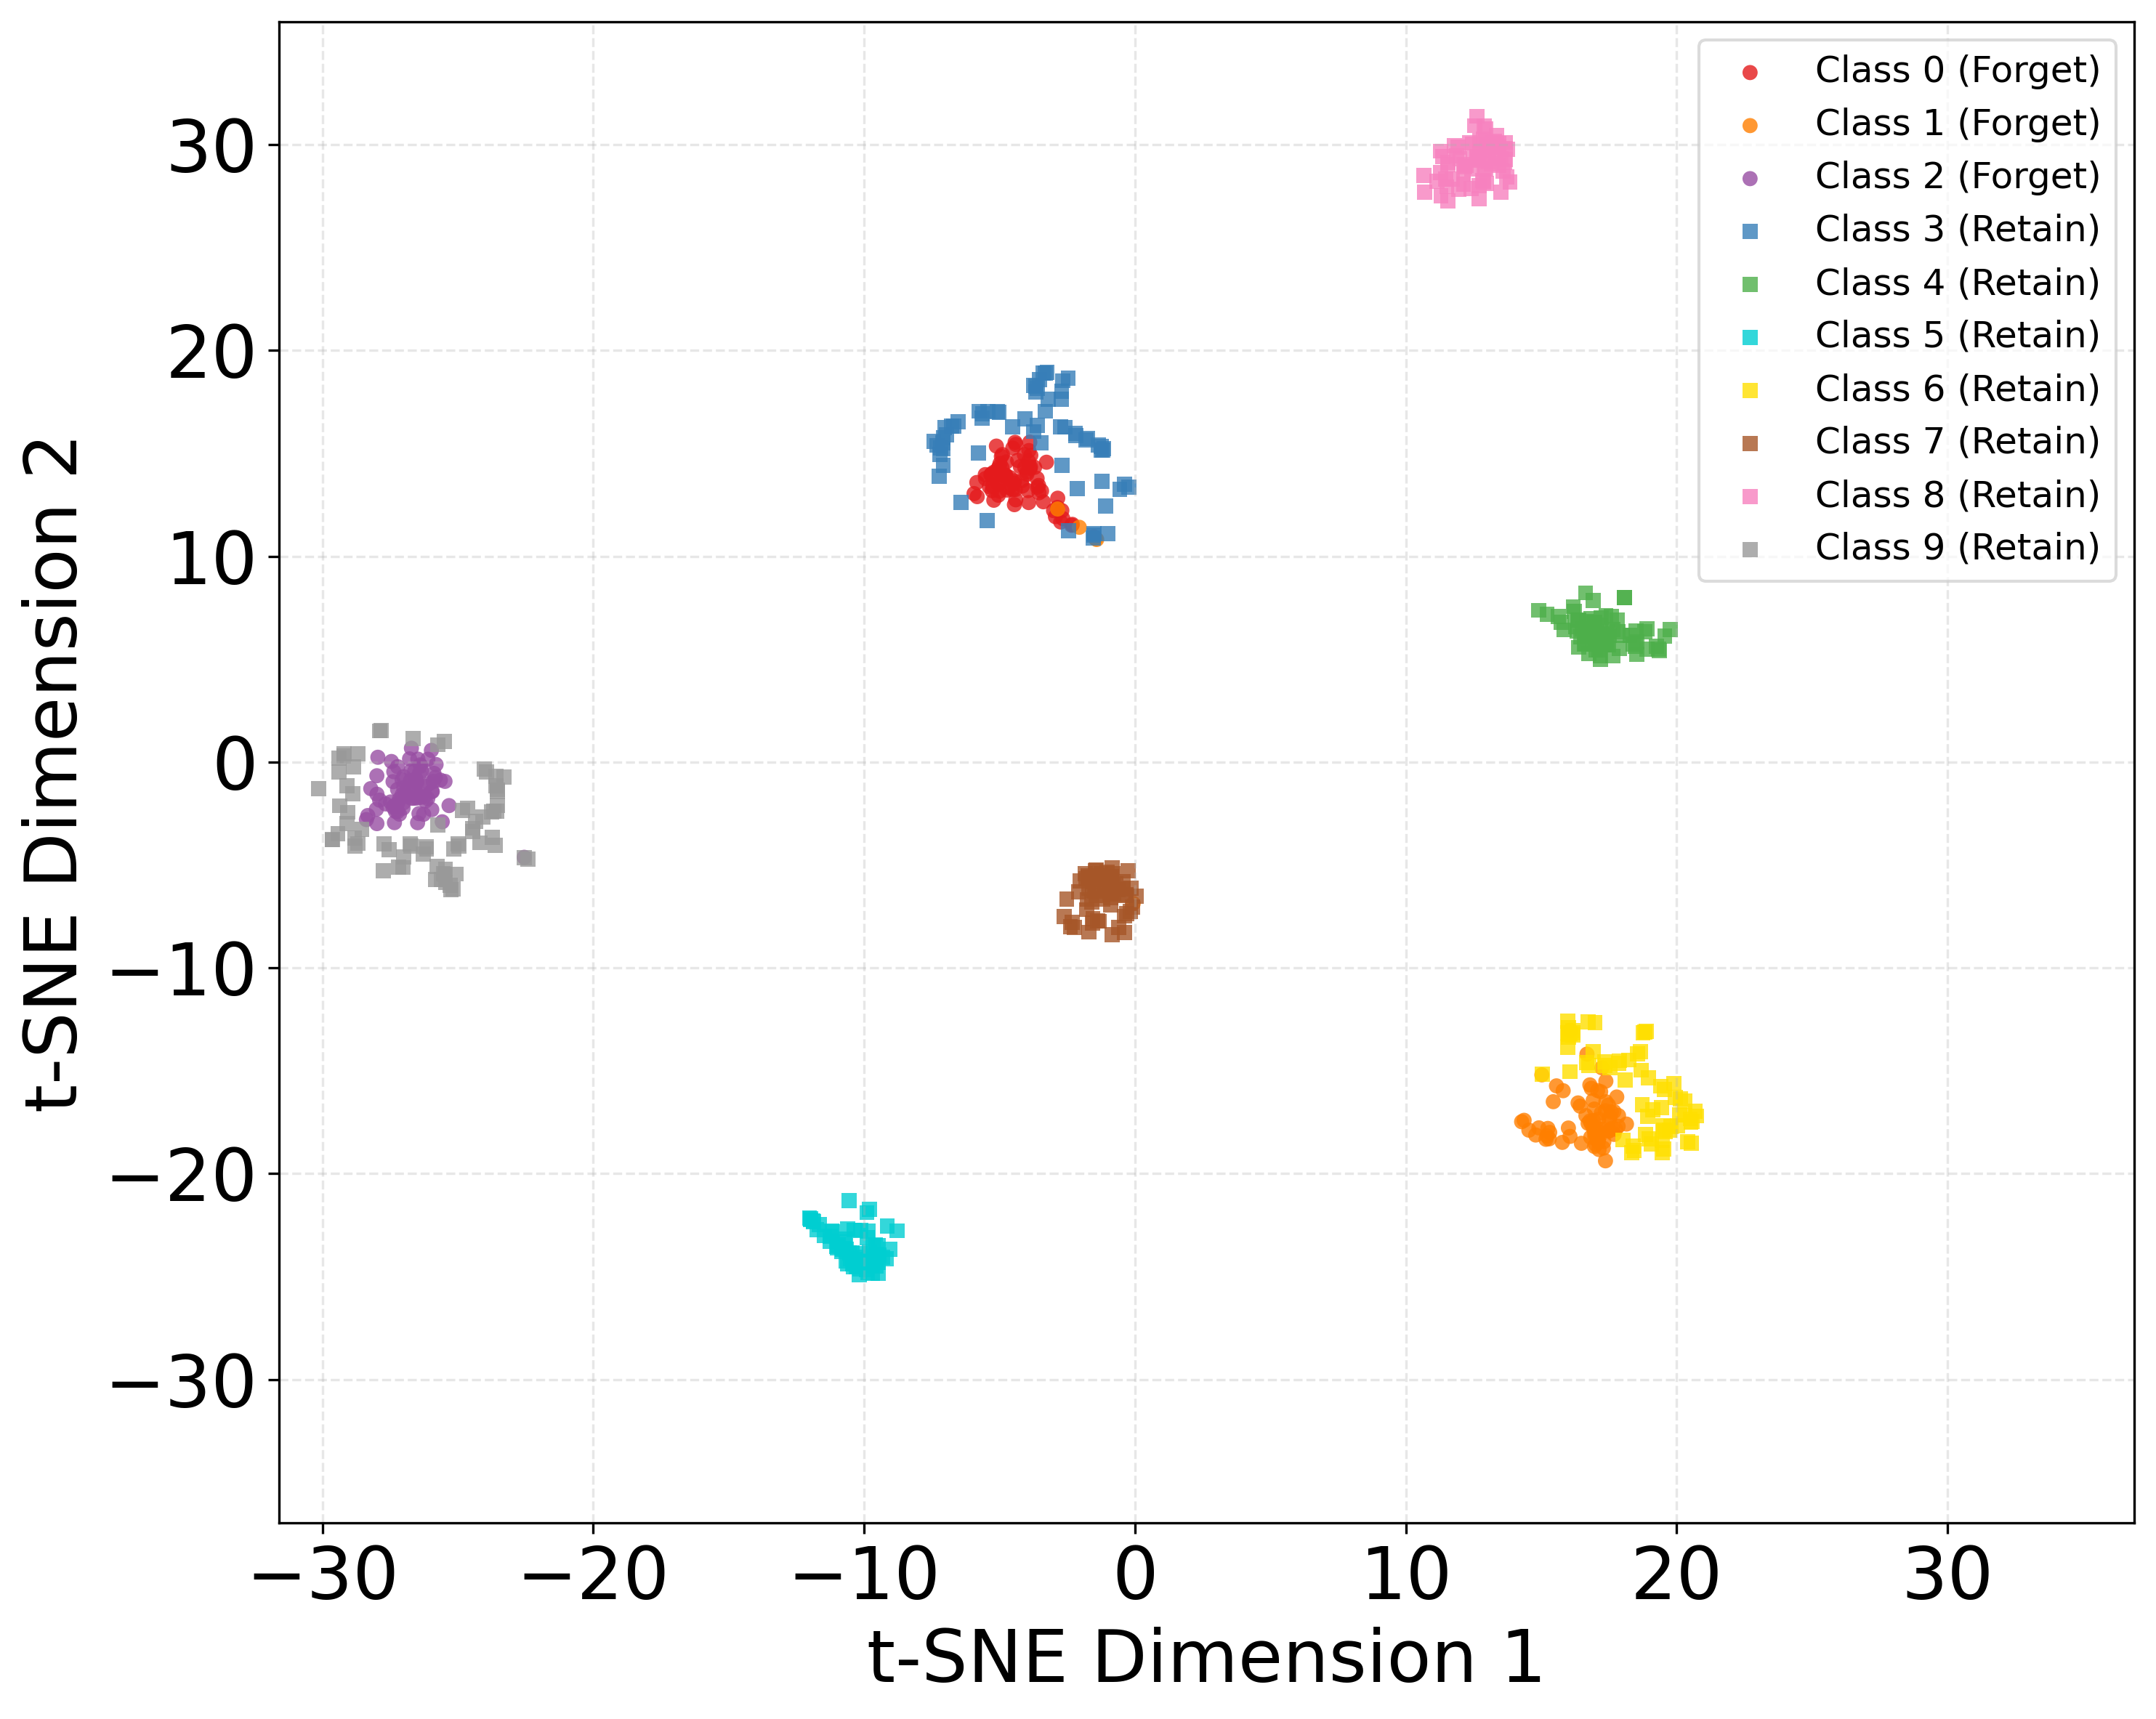
\includegraphics[width=0.45\linewidth]{tsne/cl.png}

    \vspace{0.3em}
    \makebox[0.45\linewidth]{\small (c) Boundary}
    \hfill
    \makebox[0.45\linewidth]{\small (d) CU (Ours)}

    \caption{t-SNE visualization. Baselines collapse to single point while proposed CU method distributes to nearest boundaries thus achieving faster convergence.}
    \label{fig:tsne_comparison}
\end{figure}

\subsection{Ablation Studies}
\vspace{0.2cm}
\noindent
We ablate three design choices on CIFAR-100: the replay buffer ratio $|D_\textbf{r}|$, the retain dominance constraint, and localized regularization. Table~\ref{tab:ablation_all} shows a 0.1 buffer ratio optimally balances retention and efficiency; the dominance constraint reduces $Acc_f$ from 9.97\% to 0.39\% by eliminating the long-tail convergence issue; and localized regularization reduces total $\ell_2$ norm from 39.05 to 10.09 with minimal retention loss, with Figure~\ref{fig:local_effect} showing the updates concentrate in specific blocks.

\begin{table}[!ht]
\centering
\small
\begin{tabular}{llccc}
\toprule
\textbf{Ablation} & \textbf{Setting} & $Acc_f{\downarrow}$ & $Acc_r{\uparrow}$ & \textbf{Extra} \\
\midrule
\multirow{4}{*}{Buffer Ratio $|D_r|$}
 & 1.0 (1$\times$)   & 1.33 & 74.39 & $H$=2.62 \\
 & 0.5 (2$\times$)   & 1.18 & 73.00 & $H$=2.32 \\
 & 0.3 (3.3$\times$) & 1.33 & 74.55 & $H$=2.61 \\
 & \cellcolor{orange!10}0.1 (10$\times$) & \cellcolor{orange!10}1.30 & \cellcolor{orange!10}74.52 & \cellcolor{orange!10}$H$=2.56 \\
\midrule
\multirow{2}{*}{Dominance Constraint}
 & Without & 9.97 & 78.12 & -- \\
 & \cellcolor{orange!10}With & \cellcolor{orange!10}0.39 & \cellcolor{orange!10}77.06 & \cellcolor{orange!10}-- \\
\midrule
\multirow{2}{*}{Localized Reg.}
 & Without & 0.00 & 77.24 & $\ell_2$=39.05 \\
 & \cellcolor{orange!10}With & \cellcolor{orange!10}0.00 & \cellcolor{orange!10}74.76 & \cellcolor{orange!10}$\ell_2$=10.09 \\
\bottomrule
\end{tabular}
\vspace{0.2cm}
\caption{Design ablations: replay buffer ratio, retain dominance constraint, and localized regularization on CIFAR-100. Highlighted rows are CU's default setting.}
\label{tab:ablation_all}
\end{table}

\begin{figure}[!ht]
    \centering
    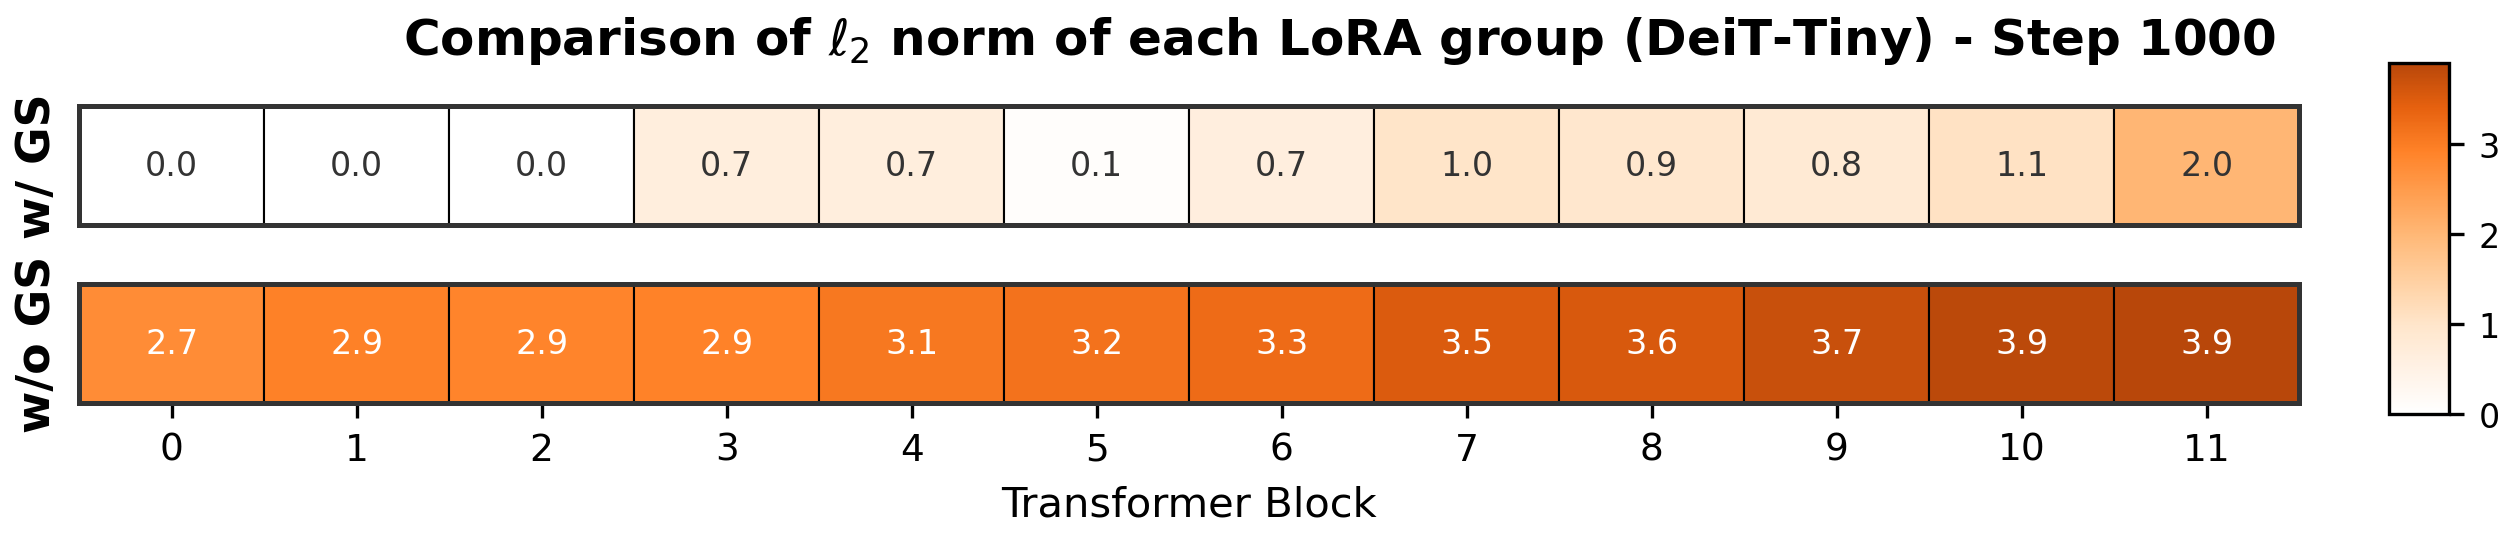
\includegraphics[width=1\linewidth]{images/GS.png}
    \caption{$\ell_2$ norm per block. Localized regularization concentrates updates in specific blocks.}
    \label{fig:local_effect}
\end{figure}

\subsection{Attack-Based Verification}
\label{sec:attack}
\vspace{0.2cm}
\noindent
\textcolor{red}{Table~\ref{tab:attack_verification}(a) reports FAR/EER of forget-class probes matched against the retain gallery on CASIA-Iris. CU tracks the Oracle closely (FAR@0.5 $3.83\%$ vs.\ $3.10\%$; EER $24.99\%$ vs.\ $21.69\%$), and both rise similarly over \textit{Before} unlearning ($1.64\%$), indicating that the small increase in open-set false accepts stems from removing the identities rather than from CU specifically.}

\textcolor{red}{Whether these residual accepts concentrate on one specific retained identity, a targeted per-identity vulnerability rather than a general accuracy shift, is a separate question. Beyond the $Acc_f$, KL, and confidence-based MIA already reported in Table~\ref{tab:all}, Table~\ref{tab:attack_verification}(b) reports six further attack-based tests on CASIA-Face100 after all forget identities are removed, each referenced against the \emph{Oracle} (retrain, information absent); values are placeholders pending final runs. The assigned-centroid match rate, each forget probe's match rate against its specifically \emph{assigned} nearest retain centroid, is no more frequent for CU than for Oracle, ruling out a concentrated, backdoor-like false-accept behavior between individual forget--retain identity pairs. The low linear-probe and slow relearning rates show forgetting is diffuse and not easily reversed, while label-only and adaptive MIA near chance and a low inversion match rate show that stronger, adaptive attacks fail as well. Results are empirical and attack-relative, not a formal guarantee, and directly support the retain-buffer necessity argument of Section~\ref{8.1}.}

\begin{table}[!ht]
\centering
\small
\setlength{\tabcolsep}{4pt}
\textcolor{red}{
\textbf{(a) FAR/EER on CASIA-Iris}\\[3pt]
\begin{tabular}{lcccc}
\toprule
Model & FAR@0.3 & FAR@0.4 & FAR@0.5 & EER \\
\midrule
Before & 11.38\% & 4.84\% & 1.64\% & 13.33\% \\
\rowcolor{orange!10}
CU & 17.97\% & 8.52\% & 3.83\% & 21.99\% \\
Oracle & 16.10\% & 7.79\% & 3.10\% & 21.69\% \\
\bottomrule
\end{tabular}
\vspace{0.3cm}
\textbf{(b) Attack-based confound tests on CASIA-Face100}\\[3pt]
\scriptsize
\begin{tabular}{lcc}
\toprule
\textbf{Test} & \textbf{CU} & \textbf{Oracle} \\
\midrule
Assigned-centroid match $\downarrow$ & \textbf{3.91} & 3.74 \\
\midrule
Linear probe (frozen emb.) $\downarrow$ & \textbf{6.28} & 4.65 \\
5-shot relearn $Acc_f$ $\downarrow$ & \textbf{5.47} & 6.12 \\
\midrule
MIA, label-only~\cite{choquette2021label} $\approx\!0.5$ & \textbf{0.53} & 0.51 \\
MIA, adaptive $\approx\!0.5$ & \textbf{0.54} & 0.50 \\
Model inversion match $\downarrow$ & \textbf{3.62} & 3.98 \\
\bottomrule
\end{tabular}}
\vspace{0.15cm}
\caption{\textcolor{red}{Attack-based verification. (a) FAR/EER of forget-class probes against the retain gallery on CASIA-Iris. (b) Six further attack-based tests on CASIA-Face100, complementing the $Acc_f$, KL, and MIA results of Table~\ref{tab:all}. Values in (b) are placeholders pending final runs.}}
\label{tab:attack_verification}
\end{table}

\section{Results Discussion}

\subsection{On the Necessity of the Retain Buffer}
\label{8.1}
A natural concern for Camouflage Unlearning is whether maintaining the replay buffer $D_r \subset D_r^{\text{full}}$ contradicts GDPR and CCPA mandates on data erasure. We argue that $D_r$ is fundamentally unavoidable for preserving task-critical knowledge, since without architectural support such as modular pathways, all parameters are jointly adjusted using both $D_f$ and $D_r^{\text{full}}$ during pretraining, making disentanglement infeasible without $D_r$ access.

Attempts to bypass $D_r$ are limited. Impair and repair methods~\cite{tarun2023fast} still require $D_r$ for repair, while source-free unlearning~\cite{ahmed2025towards} estimates retain data Hessians from $D_f$ alone but is restricted to convex losses and linear classifiers, making it inapplicable to transformers and ResNets. All established non-convex methods critically rely on $D_r$, whether through Fisher information or saliency~\cite{kirkpatrick2017overcoming,fan2023salun}, explicit retention losses~\cite{kurmanji2023towards,zhao2024continual}, or continual unlearning mechanisms such as mnemonic codes, task embeddings, experience replay, and stability regularizers~\cite{shibata2021learning,adhikari2025unlearning,liu2022continual,chatterjee2024unified,huang2025unified}.

Generative tasks offer exceptions such as FLAT~\cite{wang2024llm} and ESD~\cite{gandikota2023erasing}, which avoid $D_r$ via regularizers or teacher-generated samples, but few practical approaches eliminate $D_r$ for non-convex deep learning without sacrificing retention. Camouflage Unlearning therefore retains a minimal $D_r$ (at most $10\%$ of $D_r^{\text{full}}$), consistent with limited lawful processing allowances under GDPR and CCPA for limited lawful processing necessary to fulfill erasure obligations. \textcolor{red}{$D_r$ contains at least one sample per retain identity ($\approx$42 for classification, $\approx$32 for face, 1--2 for iris, 1 for fingerprint); all reported retain metrics are computed on the full held-out test split of $D_r^{\text{full}}$, not on $D_r$ itself, so retention performance is not measured on the samples used for replay. Furthermore, $D_r$ holds only consenting retain identities: a withdrawal request is handled as a forget request, and the buffer is refilled from the remaining consenting pool, keeping the replay mechanism consistent with limited lawful processing under GDPR and CCPA.}
\section{Conclusion}
To our knowledge, we are among the earliest to address machine unlearning for privacy-critical biometric systems, including fingerprint, iris, and face recognition. We observed that existing methods suffer from prolonged convergence due to many-to-one embedding collapse, which is particularly inefficient for biometric models experiencing frequent unlearning requests on edge devices. To address this, we propose Camouflage Unlearning, achieving up to 4$\times$ speedup through many-to-many distribution and surgical parameter modifications while delivering competitive forgetting, retention, and privacy performance comparable to state-of-the-art methods. Future work includes extending Camouflage Unlearning to continual forgetting scenarios in pretrained biometric models.

%% Acknowledgment — hide during review if needed
% \section*{Acknowledgment}
% The authors would like to thank ...

\bibliographystyle{IEEEtran}
\bibliography{ref}

\end{document}